\documentclass{article}
\usepackage{graphicx} % Required for inserting images
\usepackage{amsmath}
\usepackage{url}

\title{Assignment 4}
\author{Name : YASH SHAJIL \\Roll No. : AE22B110 \\Github user ID : YashShajil}
\date{}

\begin{document}

\maketitle

\section*{AE22B110 \\ Laplace Transform}

\subsection*{History}

The Laplace transform is named after mathematician and astronomer Pierre-Simon, marquis de Laplace.
Laplace wrote extensively about the use of generating functions (1814), and the integral form of the Laplace transform evolved naturally as a result. ~\cite{enwiki:1158213292}

\begin{figure}[h]
    \centering
    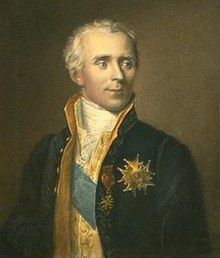
\includegraphics[width = 0.4 \textwidth]{Laplace,_Pierre-Simon,_marquis_de.jpg}
    \caption{Pierre-Simon, marquis de Laplace}
    \label{Pierre-Simon, marquis de Laplace}
\end{figure}

\subsection*{Application}

Laplace Transform is used in the processing of data signals during their transmission. Its a method for solving initial value problems in differential equations. 

\subsection*{Formula}

Laplace Transform:~\cite{oppenheim1997signals}\footnote{This formula is for the Bilateral version of Laplace Transform} 

\medskip

\begin{equation*}
    \mathcal{L}\{x(t)\} = X(s) = \int_{-\infty}^{\infty} x(t)e^{-st}\, dt\
\end{equation*}

Inverse Laplace Transform:

\medskip

\begin{equation*}
    \mathcal{L}^{-1}\{X(s)\} = x(t) = \frac{1}{2\pi j} \int_{\sigma - j\infty}^{\sigma + j\infty} X(s)e^{st}\, ds\
\end{equation*}

\medskip

where Re\{s\} = $\sigma$ is in the ROC of X(s).
This equation is solved using \textbf{Contour Integration} because s is complex. ~\cite{adams2013lecture}

\subsection*{Radius of Convergence (ROC)}\footnote{URL : https://www.tutorialspoint.com/signals\_and\_systems/region\_of\_convergence.htm}

The range variation of $\sigma$ for which the Laplace transform converges is called region of convergence.

\begin{figure}[h]
    \centering
    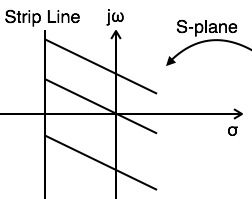
\includegraphics{strip_lines.png}
    \caption{}
    \label{fig:enter-label}
\end{figure}

\subsubsection*{Properties of ROC}

\begin{itemize}
    \item ROC contains strip lines parallel to j$\omega$ axis in s-plane.
    \item If x(t) is absolutely integral and it is of finite duration, then ROC is entire s-plane.
    \item If x(t) is a right sided sequence then ROC : Re\{s\} $>$ $\sigma_o$ .
    \item If x(t) is a left sided sequence then ROC : Re\{s\} $<$ $\sigma_o$.
    \item If x(t) is a two sided sequence then ROC is the combination of two regions.
\end{itemize}

\subsection*{Reason for choosing this equation}

Laplace Transform is a major tool in signals and systems. It is used vastly in the Aerospace field in \textbf{control systems} and \textbf{feedback mechanisms}. It makes the analysis of the system much more easier. It has huge role in automation of stuffs that we see around us all the time.

\bibliographystyle{plain}
\bibliography{refs.bib}

\end{document}
